%------------------ vorlage.tex ------------------------------------------------
%
% LaTeX-Vorlage zur Erstellung von Projektdokumentationen
% im Fachbereich Informatik der Hochschule Trier
%
% Basis: Vorlage 'svmono' des Springer Verlags
% Bearbeiter: Hermann Schloß, Christian Bettinger
%
%-------------------------------------------------------------------------------


%------------------ Präambel ---------------------------------------------------
\documentclass[envcountsame, envcountchap, deutsch]{i-studis}

\usepackage[utf8]{inputenc}

\usepackage[a4paper]{geometry}
\usepackage[english, ngerman]{babel}

\usepackage[pdftex]{graphicx}
\usepackage{epstopdf}

\usepackage{listings}

\usepackage[german, ruled, vlined]{algorithm2e}
\usepackage{amssymb, amsfonts, amstext, amsmath}
\usepackage{array}
\usepackage[skip=10pt]{caption}
\usepackage[usenames, dvipsnames]{color}
\usepackage[pdftex, plainpages=false]{hyperref}
\usepackage{textcomp}

\usepackage{bibgerm}
\bibliographystyle{geralpha}

\usepackage{makeidx}
\usepackage{multicol}
\makeindex

\pagestyle{myheadings}
\setlength{\textheight}{1.1\textheight}

\lstset{
	basicstyle=\scriptsize\ttfamily,
	commentstyle=\scriptsize\ttfamily\color{Gray},
	identifierstyle=\scriptsize\ttfamily,
	keywordstyle=\scriptsize\ttfamily,
	stringstyle=\scriptsize\ttfamily,
	tabsize=4,
	numbers=left,
	numberstyle=\tiny,
	numberblanklines=false,
	frame=single,
	framesep=3mm,
	framexleftmargin=7mm,
	xleftmargin=10mm,
	linewidth=144mm,
	captionpos=b,
}

\usepackage[Export]{adjustbox}
\adjustboxset*{width=1\linewidth}


\hypersetup{
  pdftitle={Reinforcement Learning},
  pdfauthor={Frederic Nicolas Schneider},
  pdflang={de-DE},
  pdfsubject={Simulationstechnik und Reinforcement Learning},
}

\providecommand{\tightlist}{%
  \setlength{\itemsep}{0pt}\setlength{\parskip}{0pt}}

%------------------ Manuelle Silbentrennung ------------------------------------
\hyphenation{Ele-men-tar-ob-jek-te ab-ge-tas-tet Aus-wer-tung House-holder-Matrix Least-Squares-Al-go-ri-th-men}


%------------------ Titelseite -------------------------------------------------
\begin{document}

\title{Reinforcement Learning}
\subtitle{Simulationstechnik und Reinforcement Learning}

\author{Frederic Nicolas Schneider}

\supervisor{Prof.~Dr.~Christoph Lürig}

\address{Trier}
\submitdate{11.07.2023}

%------------------ Projektart -------------------------------------------------
%\project{Bachelor-Projektarbeit}
% \project{Bachelor-Abschlussarbeit}
% \project{Master-Projektstudium}
%\project{Master-Abschlussarbeit}
%\project{Seminar}
%\project{Hausarbeit}
\project{Simulationstechnik und Reinforcement Learning}

\mytitlepage

%------------------ Vorwort, Kurzfassung, Verzeichnisse ------------------------
\frontmatter
% \input{chapters/Vorwort}								% Vorwort (optional)
% \input{chapters/Kurzfassung}							% Kurzfassung/Abstract
\tableofcontents										% Inhaltsverzeichnis
% \listoffigures											% Abbildungsverzeichnis (optional)
% \listoftables											% Tabellenverzeichnis (optional)
% \lstlistoflistings										% Listings (optional)


%------------------ Kapitel ----------------------------------------------------
\mainmatter
\newpage

\hypertarget{erweiterung-der-simulation}{%
\chapter{Erweiterung der Simulation}\label{erweiterung-der-simulation}}

\hypertarget{ruxfcckblick-auf-die-aktuelle-simulation}{%
\section{Rückblick auf die aktuelle
Simulation}\label{ruxfcckblick-auf-die-aktuelle-simulation}}

Die Simulation wurde in drei Elementen aufgeteilt: der
Fahrstuhlsteuerung, Personensteuerung und der verbindenden Simulation.
Dabei wird in jedem Takt überprüft, ob Personen einen Fahrstuhl zu einer
Etage rufen. Ist der Fahrstuhl leer, prüft er in jedem Takt, ob er
gerufen wurde. Hat er jedoch Passagiere, so fährt er zur nächsten
Zieletage und nimmt, wenn möglich, auf dem Weg weitere Passagiere mit.

\hypertarget{die-entscheider-schnittstelle}{%
\section{Die
Entscheider-Schnittstelle}\label{die-entscheider-schnittstelle}}

Als erste Erweiterung wurde eine Entscheider-Schnittstelle erstellt, die
von der Fahrstuhlsteuerung aufgerufen wird. Diese gibt in der reinen
Simulation die Entscheidung der Scanning-Strategie zurück. Ist der
Entscheider des Reinforcement Learnings aktiviert, gibt diese
Schnittstelle eine neutrale Entscheidung zurück. Die Entscheidung der
Reinforcement Learners wurde bei der ersten Implementierung nach dem
Fahrstuhlhandlings angewendet (Abbildung \ref{elevator_RL}).

\begin{figure}
\centering
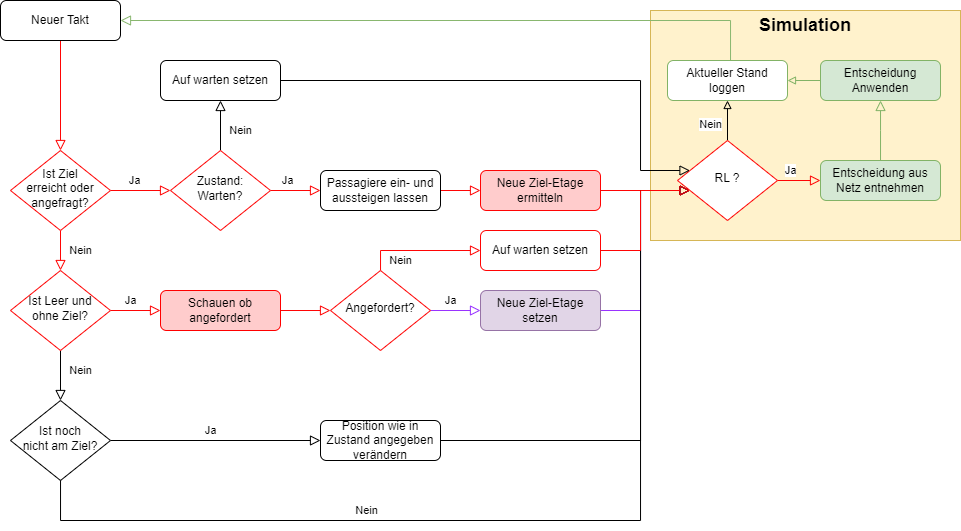
\includegraphics{../images/elevator_RL.png}
\caption{Der neue abgeänderte Ablauf der Fahrstuhlsteuerung. Entscheider
(grün), Neue Schritte (rot), Nicht mehr genutzt (lila)
\label{elevator_RL}}
\end{figure}

In einer zweiten Implementierung wurde die Möglichkeit hinzugefügt, die
Simulation nur Schrittweise auszuführen und beim Training die
Entscheidung außerhalb der Simulation zu treffen und diese für den
nächsten Takt zu übergeben. Ist nur der Entscheider dieser
Reinforcement-Implementation genutzt, so kann die Simulation diese in
jedem Takt selbstständig vom Netz anfragen.


% %------------------ Literaturverzeichnis & Index -------------------------------
% \backmatter
% \bibliography{literatur}								% Literaturverzeichnis (literatur.bib)
% \printindex												% Index (optional)


% %------------------ Anhänge ----------------------------------------------------
% \begin{appendix}
% 	\include{chapters/Glossar}							% Glossar (optional)
% 	\include{chapters/Selbststaendigkeitserklaerung}	% Selbstständigkeitserklärung
% \end{appendix}


\end{document}
